\chapter{Experimental performance analysis}
\label{Cap:Exp}
%\vspace{-1.0cm}
%

This chapter aims to analyse the outdoor experimental performance of the solar air heater prototype fabricated using the concentrator designed in Chapter \ref{Cap:Opt}. This air heating system was fabricated and tested at Technological University Dublin, Ireland. The specific objectives are to:

\begin{itemize}
	\item Present the materials and components for fabrication;
	\item Describe the data collection procedure and equipment used;
	\item Evaluate the thermal performance of the system in an open loop configuration.
\end{itemize}

\section{Materials for the prototype}
	
\subsection{Absorber surface selection}

The function of the absorber surface in solar thermal systems is to retain thermal energy from incoming solar radiation. To meet this objective, carbon fibre weave fabric has been selected as the absorbing material (Figure \ref{CFphoto}). Although it is not conventionally employed in solar air heating systems (\cite{Shams2013}), its utilisation brings two advantages: i) it has natural perforations, and ii) it reduces the system's weight -- compared to an aluminium plate of the same dimensions, the carbon fibre surface is 40\% lighter.

\Figure[scale=0.3,placement=!ht,label={CFphoto},caption={Carbon fibre weave fabric (\cite{EasyComposites2017}).}]{figs/CFphoto.PNG}

\newpage
Carbon fibre weave's physical properties are presented in Table \ref{carbonfiber}. Absorptivity data were reported by \citet{Wu2012}, whereas thermal conductivity and specific heat were obtained from the material supplier Easy Composites (\cite{EasyComposites2017}). Despite being a modest thermal conductor, \citet{Gawlik2005} reported that this factor poorly influences the thermal efficiency of an air heating system with a perforated absorber.

\begin{table}[!ht]
	\caption{Carbon fibre weave properties.}
	\centering
	\begin{tabular}{p{5cm}p{4cm}}
		\hline \\[-12pt] 
		Property & Value \\ 
		\hline \\[-12pt] 
		Thickness & 0.30 mm \\ [3pt]
		Density & 1790 kg/m$^3$ \\ [3pt]
		Thermal Conductivity & 10.42 W/(m K) \\ [3pt]
		Specific Heat & 795 J/(kg K) \\ [3pt]
		Absorptivity & 0.85 \\ [1pt]
		\hline 
	\end{tabular} 
	\label{carbonfiber}
\end{table}

The carbon fibre weave fabric is made of multi-filament yarns, and the type of weave is considered according to the application (\cite{Tourlonias2016}). The area between the woven yarns are the perforations through which the flowing air passes. This porosity was calculated from data from morphology images (Figure \ref{CFmag}) by \citet{Shams2013}. The average perforation area and porosity values are 0.147 mm$^2$ and 4.2\%, respectively, and will be input as parameters in the thermal modelling depicted in \mbox{Chapter \ref{Cap:Thermal}}. The cost of this carbon fibre weave fabric was 24 \euro/${\rm m^2}$.

\Figure[scale=0.65,placement=!ht,label={CFmag},caption={Morphology image of carbon fibre sample taken at magnification of 15x.}]{figs/CFmag}

Epoxy laminating resin was applied to the corners of the surface to assemble the carbon fibre fabric onto the prototype. This was done to prevent splitting in the weave and ensure the surface remained stretched. The corners were then secured to a thin wooden frame with specific absorber dimensions (0.145 m x 1.25 m).

\subsection{Glazing cover selection}

A glazing material that enhances light transmission and avoids optical losses is needed. For the task, the selected glazing material for this system is a 4-mm thick tempered clear glass slab. This tempered property makes the glass safer and more durable than ordinary glass. It withstands 5 times more impact before shattering. If shattered, the fragments pose a reduced danger to the user, making it an attractive product for use in both commercial and domestic applications (\cite{FirstGlass2016}). The glass properties, such as absorptivity and transmittance, are shown in Table \ref{glass_tempered}. From the collector's design, the glazing dimensions are \mbox{0.27 m x 1.25 m}. The cost of the glass was 70 \euro/${\rm m^2}$.

\begin{table}[!ht]
	\caption{Glazing cover properties.}
	\centering
	\begin{tabular}{p{5cm}p{4cm}}
		\hline \\[-12pt] 
		Property & Value \\ 
		\hline \\[-12pt] 
		Thickness & 4 mm \\ [3pt]
		Density & 2500 kg/m$^3$ \\ [3pt]
		Absorptivity\footnotemark[1] & 0.02 \\ [3pt]
		Transmittance\footnotemark[1] & 0.90 \\ [3pt]
		Specific Heat & 880 J/(kg.K)  \\ [1pt]
		\hline 
	\end{tabular} 
	\label{glass_tempered}
\end{table}

\footnotetext[1]{Values at near normal incident light}

\subsection{Reflector surface selection}

The reflective material employed is \textit{MiroSun} from the German company Alanod, the only product used for solar applications. This reflective aluminium sheet is manufactured using a continuous physical vapour deposition (PVD) process applied for a super reflective layer to coil anodised material. Afterwards, the surface is protected by a nano-composite in a coil-coating process. Table \ref{reflector_M} shows the optical and physical properties of this material. From the concentrator's design, the total area of the reflector sheet used was 1.25 m x 1.20 m. The cost of the Alanod reflector was 50 \euro/${\rm m^2}$.

\begin{table}[!ht]
	\caption{\textit{MiroSun} reflector properties (\cite{Alanod2016}).}
	\centering
	\begin{tabular}{p{5cm}p{4cm}}
		\hline \\[-12pt] 
		Property & Value \\ 
		\hline \\[-12pt] 
		%Front Side Layer & PVD improved \\ [3pt]
		%Reverse Side Layer & Anodised \\ [3pt]
		Thickness & 0.5 mm \\ [3pt]
		Density & 2700 kg/m$^3$ \\ [3pt]
		%Max. Width & 1.25 m \\ [3pt]
		Total Reflectivity & 0.95 \\ [1pt]
		\hline 
	\end{tabular} 
	\label{reflector_M}
\end{table}

\subsection{Prototype's structure}

The materials used to fabricate the prototype's structure are listed as follows:

\begin{itemize}
	\item 0.7 m$^2$ of a 2-mm thick aluminium sheet to form the ends;
	\item 8 aluminium bars of 1.25 m in length to support and keep the reflectors in the desired position;
	\item 0.45 m$^2$ of 1-cm thick timber to form a cavity above the absorber surface in order to reduce heat losses;
	\item two 2.5-in diameter aluminium pipes of 10 cm in length for the airflow inlet and outlet;
	\item 1.8 m$^2$ of a 0.6-mm thick aluminium sheet to box the whole structure.
	
\end{itemize}

Figure \ref{Ass11} shows photographs of the assembled structure. The space between the reflectors and the outer aluminium sheet was filled with fibre glass wool to provide thermal insulation. The structure was wrapped with polyurethane foam board and sealed with waterproof tape.

\begin{figure}[ht!]
	\begin{minipage}{0.49\columnwidth}
		\includegraphics[width=0.95\columnwidth,height=5cm]{figs/Ass1.jpg}
		\subcaption{One end assembled.}
		
		\includegraphics[width=0.95\columnwidth,height=5cm]{figs/Ass2.jpg}
		\subcaption{Two ends and aluminium bars assembled.}
	\end{minipage}
	\begin{minipage}{0.49\columnwidth}
		\includegraphics[width=0.95\columnwidth,height=5cm]{figs/Ass4.jpg}
		\subcaption{Closed structure.}
		
		\includegraphics[width=0.95\columnwidth,height=5cm]{figs/Ass3.jpg}
		\subcaption{Closed structure with the glass.}
		
	\end{minipage}
	\caption{Parts of the prototype's structure and assembled}
	\label{Ass11}
\end{figure}

%\Figure[scale=0.45,placement=!ht,label={Structure1},caption={Aluminium structure of the solar air heater.}]{figs/Structure1.png}

\section{Instrumentation of the experimental unit}

Temperatures were measured at the inlet and outlet of air, absorber and glazing surfaces using type T (Cu-CuNi) PTFE insulated twist fine wire thermocouple sensors with an accuracy of $\pm$0.5 $^{\rm{o}}$C. Figures \ref{TC_abs} and \ref{TC_glaz} indicate the position of each thermocouple on the absorber and glazing surfaces, respectively. 18 thermocouples were used in total. As a matter of orientation, in both figures, the side where the thermocouple 1 is placed is the closest to the outlet.

\Figure[scale=0.50,placement=!ht,label={TC_abs},caption={Positions of the 12 thermocouples numbered from 1 to 12 placed on the absorber surface (dimensions in mm).}]{figs/absorber_thermocouple.PNG}

\Figure[scale=0.40,placement=!ht,label={TC_glaz},caption={Position of the three thermocouples numbered from 1 to 3 placed on the glazing surface (dimensions in mm).}]{figs/glass_thermocouple.PNG}

These temperature measurements were recorded at 1-minute intervals with a DL2e data logger connected directly to a computer, where the temperature data were downloaded via a USB port (\cite{Devices2018}). All thermocouples were labelled, inserted in a plug and connected to the data logger.

\newpage
The airflow was provided by a 12-W fan, where the rate was varied by a voltage adaptor with five different voltage inputs. The air velocity at the air outlet ($\rm{v_{in}}$, in m/s) was measured using a Testo 425 hot wire anemometer. These velocity levels were converted to airflow values using Eq. (\ref{Gpitot}).

%\begin{equation}
%\mathrm{{v_{out}} = \sqrt {\frac{{2{\mathrm{P_{out}}}}}{{{\mathrm{d_{air}}}}}}}
%\label{Vpitot}
%\end{equation}

\vspace{-0.75cm}
\begin{equation}
\mathrm{{G_{air}} = \frac{{{v_{in}}{A_{out}}{d_{air}}}}{{{A_{abs}}}}}
\label{Gpitot}
\end{equation}

\noindent where $\rm{A_{out}}$ is the cross-section area of the outlet pipe (m$^2$), $\rm{d_{air}}$ is the air density (kg/m$^3$) and  $\rm{G_{air}}$ is the mass airflow rate per absorber area (kg/(s.m$^{{\rm{2}}}$)).

The measured variables are subjected to systematic uncertainties due to instrumentation errors. It is thus necessary to calculate the standard uncertainty of each variable measured for the experimental work. Those measurements are temperature, air velocity and solar radiation. The accuracy of each instrument, taken from the manufacturer data is shown in Table \ref{uncertainty}.   

\begin{table}[!ht]
	\caption{Measurements and standard uncertainty.}
	\centering
	\begin{tabular}{p{3.0cm}p{3.5cm}p{3.5cm}}
		\hline \\[-10pt] 
		\rule[-1ex]{0pt}{2.5ex} Measurement & Accuracy & Uncertainty \\ [3pt]
		\hline \\[-10pt]
		\rule[-1ex]{0pt}{2.5ex} Temperature & ${\rm \pm0.55 ^{\rm o}C \pm0.3 ^{\rm o}C}$ & 0.36 $^{\rm o}$C \\ [5pt]
		\rule[-1ex]{0pt}{2.5ex} Air velocity &  $\pm$(0.03 + 5\% of ${\rm v_{in})}$ & 0.0173 + 0.0289${\rm v_{in}}$ \\ [5pt] 
		%\rule[-1ex]{0pt}{2.5ex}  & 0.070 & 650 \\ [5pt]
		%\rule[-1ex]{0pt}{2.5ex} 8.70 & 0.090 & 820 \\ [5pt]
		\rule[-1ex]{0pt}{2.5ex} Solar radiation & -- & 1\% of ${\rm I_{\!_T}}$ \\ [2pt]
		\hline 
	\end{tabular}
	\label{uncertainty}
	
\end{table}


\newpage
Table \ref{GxV} shows the air velocity and airflow rate values as a function of the voltage input input ($\rm{V_a}$) and a category corresponding to each level. Systematic uncertainties were also calculated for the airflow rate (${\rm u_g}$).

\begin{table}[!ht]
	\caption{Mass and volumetric flow rates calculated at each voltage input.}
	\centering
	\begin{tabular}{p{2.1cm}p{1.8cm}p{2.4cm}p{2.2cm}p{1.8cm}}
		\hline \\[-10pt] 
		\rule[-1ex]{0pt}{2.5ex} Voltage (V) & ${\rm v_{in}}$ (m/s) & $\rm{G_{air}}$ (kg/m$^2$.s) & ${\rm u_{g}}$ (kg/m$^2$.s)  & Code \\ [3pt]
		\hline \\[-10pt]
		\rule[-1ex]{0pt}{2.5ex} 4.92 & 1.83 & 0.038 & 0.0021 & Low\\ [5pt]
		\rule[-1ex]{0pt}{2.5ex} 5.82 & 2.59 & 0.054 & 0.0030 & Low-med \\ [5pt] 
		\rule[-1ex]{0pt}{2.5ex} 7.20 & 3.43 & 0.071 & 0.0039 & Medium \\ [5pt]
		\rule[-1ex]{0pt}{2.5ex} 8.70 & 4.30 & 0.089 & 0.0048 & Med-high  \\ [5pt]
		\rule[-1ex]{0pt}{2.5ex} 11.30 & 5.50 & 0.114 & 0.0060 & High \\ [2pt]
		\hline 
	\end{tabular} 
	\label{GxV}
\end{table}

%Hence, a 2$^{\rm{nd}}$ degree polynomial was fit from the previous data, as shown in \mbox{Eq. (\ref{Gfit}):} 

%\begin{equation}
%\mathrm{{G_{air}} =  - 6.3 \cdot {10^{ - 4}}V_a^2 + 0.022V_a - 0.054}
%\label{Gfit}
%\end{equation}

%The pressure drop across the prototype was calculated at each airflow level and are presented in Figure \ref{dP-Gair}.

%\Figure[scale=0.50,placement=!ht,label={dP-Gair},caption={Pressure drop for different mass airflow rates}]{figs/dP-Gair.eps}

An open-loop experimental system diagram is shown in Figure \ref{scheme_p}. A flexible duct was connected to the prototype's inlet. The fan flowed air through the duct to the collector. The power supply unit provided voltage to the fan and energy to the data logger.

\Figure[scale=0.90,placement=!ht,label={scheme_p},caption={Schematic diagram of the experimental unit.}]{figs/scheme_prototype.png}

Figure \ref{unit1} presents the prototype's front view. It was fixed to the ground to prevent it from moving due to severe wind conditions. The fan was enclosed and protected from the environment during the experiments, and the data logger was placed behind the prototype.

\Figure[scale=0.48,placement=!ht,label={unit1},caption={Open-loop outdoor prototype.}]{figs/unit3.png}

\section{Experimental results from the air heating prototype}

This section presents the experimental results from tests conducted at the five airflow rates and those without flow. The thermal performance of the prototype focused on evaluating the useful energy rate (or energy delivered), collector thermal efficiency and outlet air temperature. The useful heat rate transferred to the airflow is estimated by Eq. (\ref{usefulenergy}) (\cite{Kalogirou2004}) using temperature measurements from the inlet and outlet:

\vspace{-0.75cm}
\begin{equation}
\mathrm{{Q_u} = {G_{air}}{A_{abs}}{C_{p,air}}({T_{out}} - {T_{in}})}
\label{usefulenergy}
\end{equation}

The thermal efficiency, which is the ratio of useful heat rate to the incoming total solar radiation on the aperture, is calculated by Eq. (\ref{ThermalEf0}). The solar radiation data used in the calculations were downloaded from the Met Eireann website (\cite{MetEireann2018}). Such data were measured by a solar pyranometer placed at the horizontal.

\subsection{Experimental results at transient state}

Experimental results of measured temperatures and solar radiation were used to calculate energies and thermal efficiency hourly. One day of each level of airflow rate was taken for data treatment and discussion, from 9:00 to 17:00 in 2018. 

\subsubsection{Experimental results at zero airflow}

The equilibrium temperature that the absorber approaches when no energy is removed from the collector is known as the stagnation temperature (\cite{Rabl1985}). To verify this condition, the system's inlet and outlet were closed, and two tests were conducted on clear sky days, specifically on 2$^{\rm{nd}}$ and 3$^{\rm{rd}}$ July, as shown in Figure \ref{zero12}. The temperature profile of the absorber represents the average measurements from all 12 thermocouples placed on its surface. During both tests, peaks of maximum stagnation absorber temperatures reached 77 $^{\rm{o}}$C with an average $\rm{I_{\!_T}}$ of 830 W/m$^{\rm{2}}$ and $\rm{T_{amb}}$ of 22 $^{\rm{o}}$C occuring around 14:00 on both days.

\Figure[scale=0.70,placement=!ht,label={zero12},caption={Experimental results from 2$^{\rm{nd}}$ and 3$^{\rm{rd}}$ July at zero airflow.}]{figs/zero12.eps}

Figure \ref{thermocouples} shows the measured temperatures for each thermocouple positioned on the absorber surface in order to investigate the stagnation point. The temperatures at the left end (T10/T11/T12) are slightly higher than those at the right (T1/T2/T3). This difference can be attributed to the fact that at 14:00 on 2$^{\rm nd}$ July, the Sun's altitude and azimuth angles are 59$^{\rm o}$ and 14\textdegree. Consequently, a concentration of energy may be occurring on the left side, which explains the temperature variation. Another observation is that the energy flux was well distributed along the area, as most temperatures are near the average value.

\Figure[scale=0.40,placement=!ht,label={thermocouples},caption={Temperatures measured by the thermocouples on the absorber surface.}]{figs/thermocouples.png}

This result can be compared to the energy distribution obtained by the ray tracing algorithm used in Chapter 3 and shown in Figure \ref{case_ch4}. The analysis indicates that the left end of the absorber surface received significantly more energy compared to the right end, which is clearly reflected in the corresponding measured temperatures. In particular, the higher temperatures at the left end suggest that it is more effectively absorbing energy. Conversely, although the right end does not receive direct radiation, its temperatures are still relatively close to the average. This suggests that some level of energy redistribution or thermal conduction may be occurring. In summary, this analysis provides a means to validate the previously developed optical modelling.

\Figure[scale=0.40,placement=!ht,label={case_ch4},caption={Energy distribution on the absorber surface obtained via ray tracing, where the Sun's altitude and azimuth angles are 59$^{\rm o}$ and 14\textdegree.}]{figs/case_ch4.eps}

\newpage
\subsubsection{Experimental results with airflow}

The findings of a low airflow rate (0.038 kg/m$^2$.s) experiment are presented in Figure \ref{004}. It was conducted on 9$^{\rm{th}}$ June under clear sky conditions with the highest solar radiation values at the solar noon hour (13:00 -- 14:00), where its peak is 860 W/m$^2$. During this hour, the average outlet airflow temperature $\rm{T_{out}}$, ambient temperature $\rm{T_{amb}}$, and thermal efficiency $\eta_{\rm{th}}$ were observed to have average values of 51 $^{\rm{o}}$C, 23 $^{\rm{o}}$C, and 0.53, respectively. At around the peak of solar radiation, the maximum $\rm{T_{out}}$ was found to be 51~$^{\rm{o}}$C, resulting in an airflow temperature rise of 28 $^{\rm{o}}$C and a corresponding $\eta_{\rm{th}}$ of 0.54. The total incident solar radiation received during the test was estimated to be 20.46 MJ/m$^2$, of which a total useful energy collected $\rm{Q_{u}}$ of 7.64 MJ/m$^2$ was calculated, resulting in a daily thermal efficiency of 0.35.

\begin{figure}[!ht]
	\centering
	\begin{minipage}{0.49\textwidth}
		\centering
		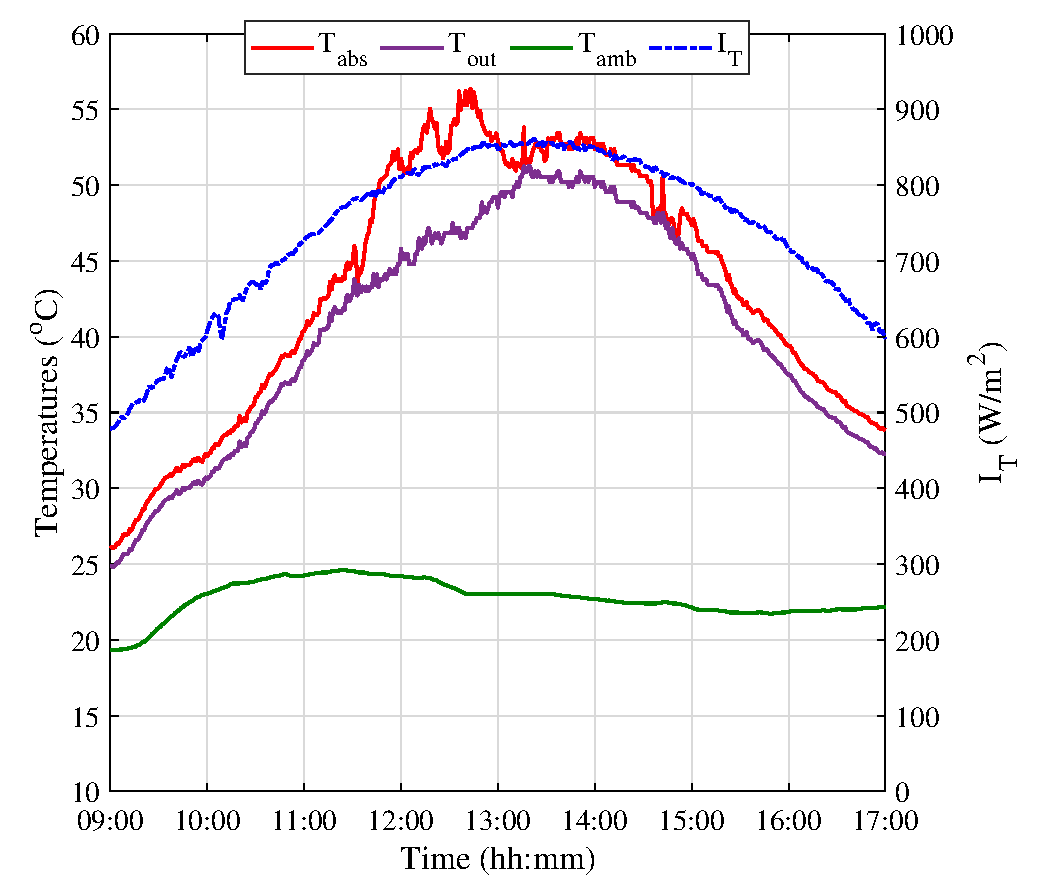
\includegraphics[width=0.98\textwidth]{figs/004-1.eps} % first figure itself
		\subcaption{Temperature results and solar data.}
	\end{minipage}\hfill
	\begin{minipage}{0.49\textwidth}
		\centering
		\includegraphics[width=0.98\textwidth]{figs/004-2.eps} % second figure itself
		\subcaption{Hourly performance and solar data.}
	\end{minipage}

	\caption{Experimental results from 9$^{\rm{th}}$ June at 0.038 kg/(s m$^2$).}
	\label{004}
\end{figure}

The results of an experiment conducted at a low-medium airflow rate (0.055 kg/m$^2$.s) under relatively clear sky conditions are depicted in Figure \ref{0055}. During the solar noon hour (13:00 -- 14:00), the airflow collected 1.7 MJ/m$^2$ of energy at an average outlet temperature of 43 $^{\rm{o}}$C and thermal efficiency of 55\%. The highest outlet temperature ($\rm{T_{out}}$) was recorded as 42 $^{\rm{o}}$C when the ambient temperature ($\rm{T_{amb}}$) was 20 $^{\rm{o}}$C, resulting in a maximum temperature rise of 22 $^{\rm{o}}$C. The total solar energy available was 21.29 MJ/m$^2$, while the total useful energy collected was 9.56 MJ/m$^2$. The thermal efficiency obtained for this day was 43\%.

%The highest outlet temperature ($\rm{T_{out}}$) was recorded as 43 $^{\rm{o}}$C when the ambient temperature ($\rm{T_{amb}}$) was 21 $^{\rm{o}}$C. The maximum temperature rise of the airflow was observed to be 22 $^{\rm{o}}$C, and the corresponding thermal efficiency ($\eta_{\rm{th}}$) during this period was estimated at 55\%. The total solar energy available was 21.29 MJ/m$^2$, while the total useful energy collected was 9.56 MJ/m$^2$. The thermal efficiency obtained for this day was 43\%. During the solar noon hour (13:00 -- 14:00), the airflow collected 1.7 MJ/m$^2$ of energy at an average outlet temperature of 43 $^{\rm{o}}$C.

%The experimental results of this test operating at low-med airflow (0.055 kg/m$^2$.s) are shown in Figure \ref{0055} under relatively clear sky condition. The highest $\rm{T_{out}}$ measured was 43 $^{\rm{o}}$C  when $\rm{T_{in}}$ = 23 $^{\rm{o}}$C and $\rm{T_{amb}}$ = 21 $^{\rm{o}}$C. The maximum airflow temperature rise was 20 $^{\rm{o}}$C observed between 13:00 and 14:00. The thermal efficiency ($\eta_{\rm{th}}$) on this same region was 55\%. The total solar energy available on 22$^{\rm{nd}}$ June was 21.29 MJ/m$^2$; the total useful energy collected was 9.56 MJ/m$^2$; and the thermal efficiency for this day obtained was 43\%. In the hour of solar noon (13h -- 14h), the airflow collected 1.7 MJ/m$^2$ of energy at an average $\rm{T_{out}}$ of 43 $^{\rm{o}}$C.


\begin{figure}[!ht]
	\centering
	\begin{minipage}{0.49\textwidth}
		\centering
		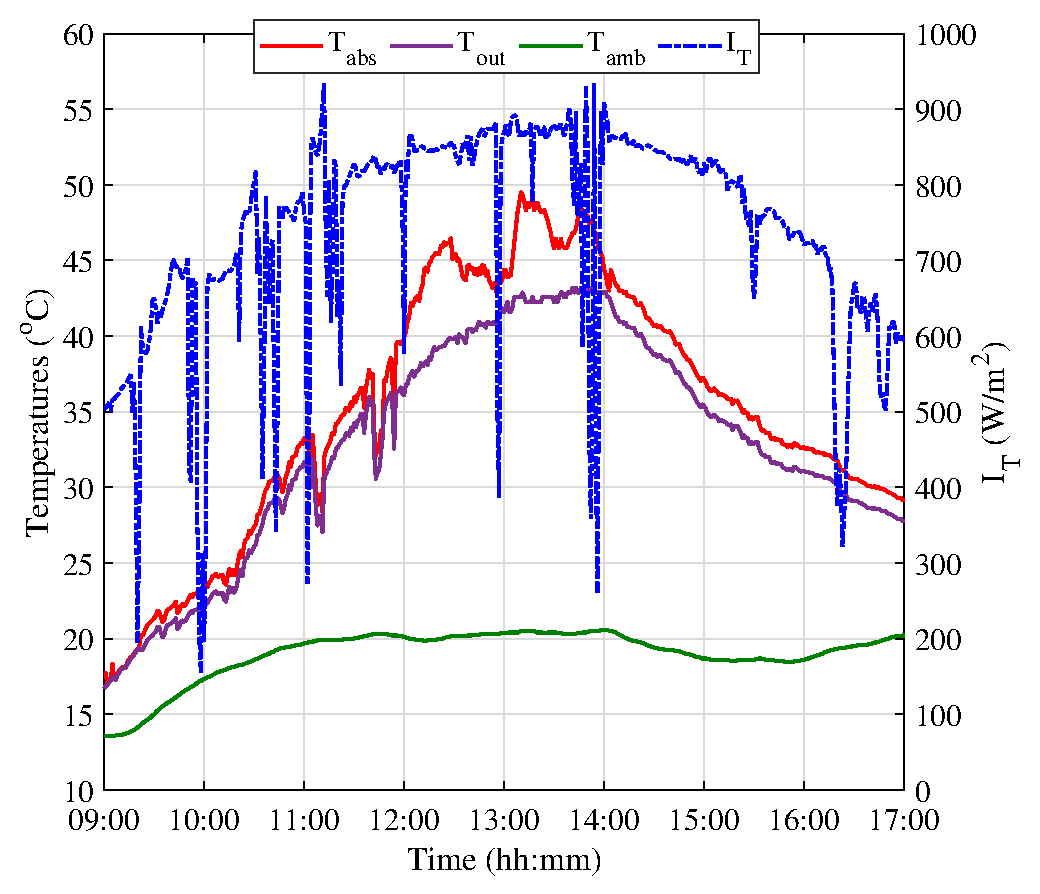
\includegraphics[width=0.98\textwidth]{figs/0055-1.eps} % first figure itself
		\subcaption{Temperature results and solar data.}
	\end{minipage}\hfill
	\begin{minipage}{0.49\textwidth}
		\centering
		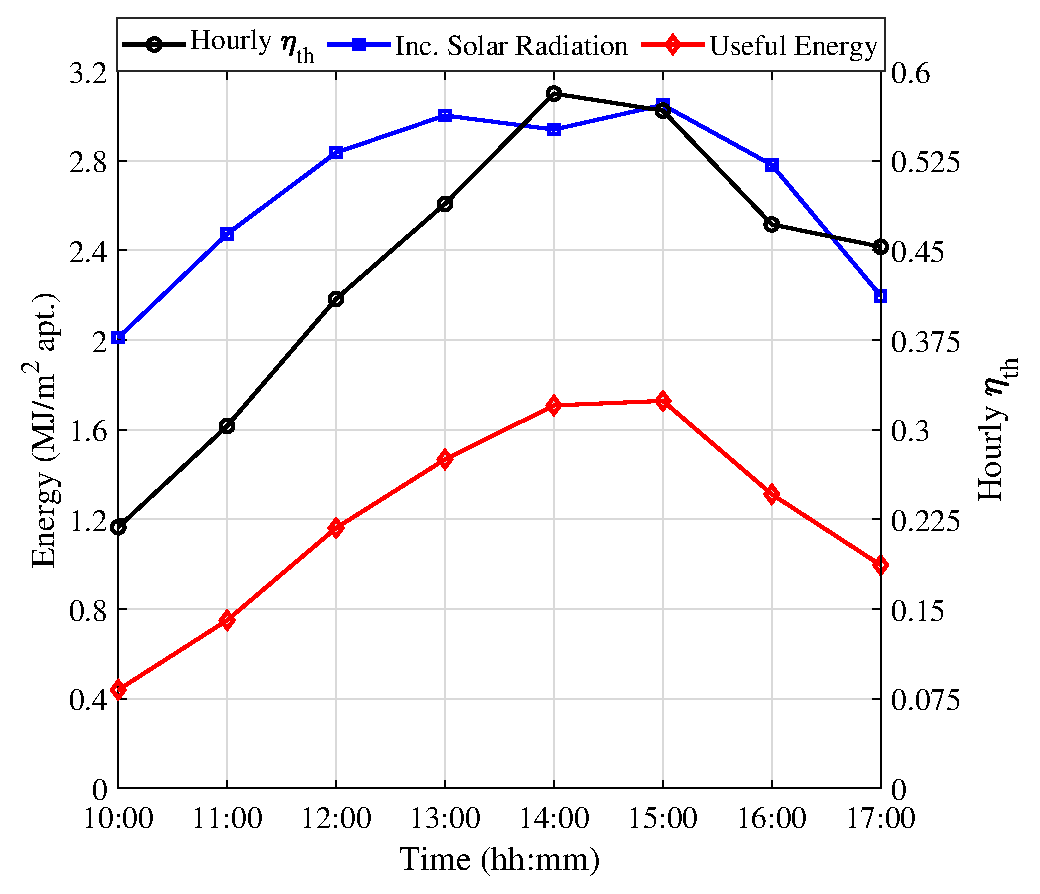
\includegraphics[width=0.98\textwidth]{figs/0055-2.eps} % second figure itself
		\subcaption{Hourly performance and solar data.}
	\end{minipage}
	
	\caption{Experimental results from 22$^{\rm{nd}}$ June at 0.054 kg/(s m$^2$).}
	\label{0055}
\end{figure}

The experimental results of the test operating at medium airflow (0.07 kg/m$^2$.s) are shown in Figure \ref{007} on 29$^{\rm{th}}$ May, in relatively clear sky conditions. The highest $\rm{T_{out}}$ was measured to be 41 $^{\rm{o}}$C  when $\rm{T_{amb}}$ was 21 $^{\rm{o}}$C. The maximum airflow temperature rise was 20 $^{\rm{o}}$C observed between 13:00 and 14:00. The thermal efficiency ($\eta_{\rm{th}}$) in this region was 58\%. The total incident solar energy available on this day was 21.4 MJ/m$^2$; the total useful energy collected was 10.03 MJ/m$^2$, and the average thermal efficiency obtained was 46\%. In the hour of highest solar radiation, the airflow collected 1.7 MJ/m$^2$ of energy at an average $\rm{T_{out}}$ of 40 $^{\rm{o}}$C.


\begin{figure}[!ht]
	\centering
	\begin{minipage}{0.49\textwidth}
		\centering
		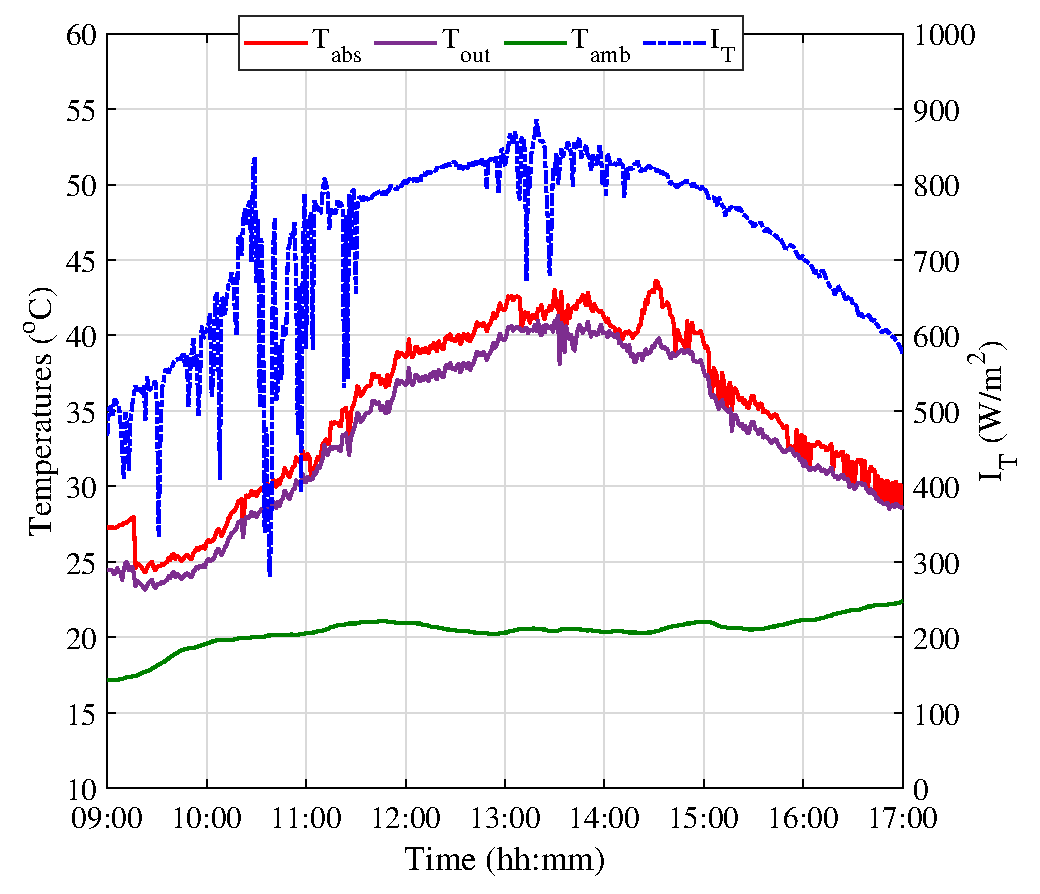
\includegraphics[width=0.98\textwidth]{figs/007-1.eps} % first figure itself
		\subcaption{Temperature results and solar data.}
	\end{minipage}\hfill
	\begin{minipage}{0.49\textwidth}
		\centering
		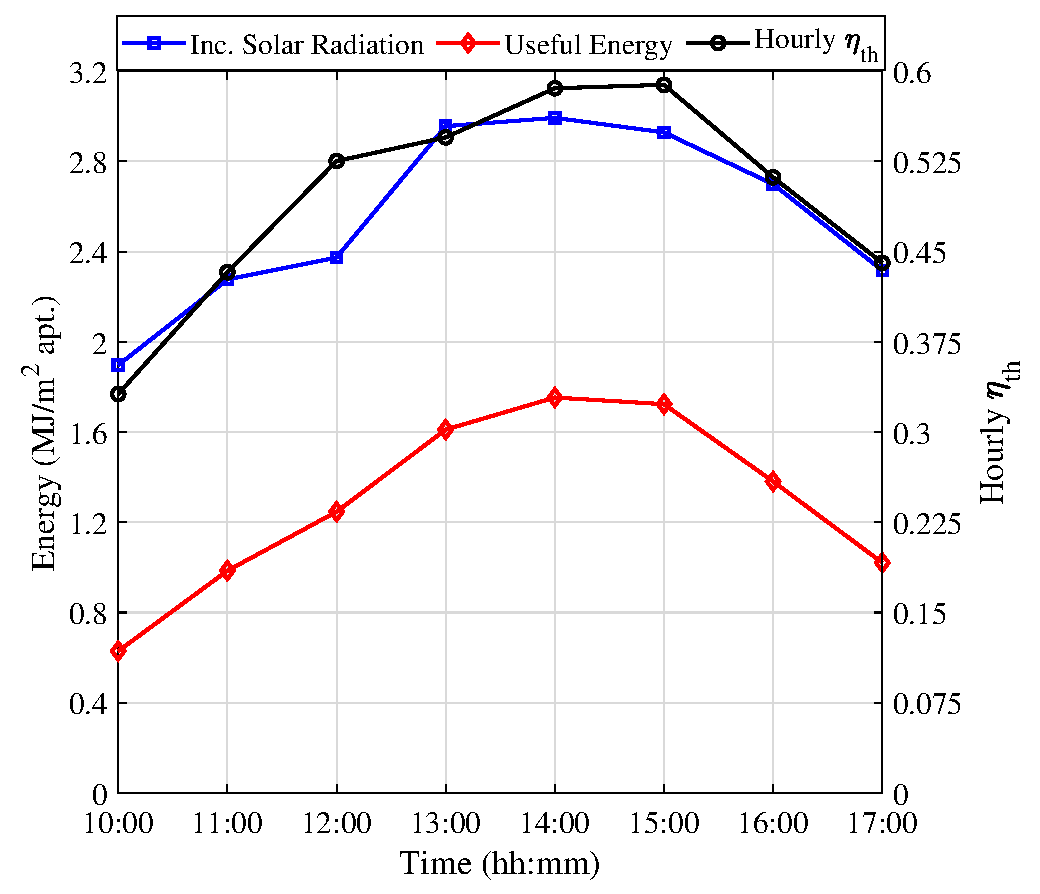
\includegraphics[width=0.98\textwidth]{figs/007-2.eps} % second figure itself
		\subcaption{Hourly performance and solar data.}
	\end{minipage}
	
	\caption{Experimental results from 29$^{\rm{th}}$ May at 0.071 kg/(s m$^2$).}
	\label{007}
\end{figure}

\newpage
The results of the test at med-high airflow (0.089 kg/m$^2$.s) are shown in Figure \ref{009} on 31$^{\rm{st}}$ May. Although the solar data is very transient on this day, $\rm{T_{out}}$ kept constant around 39 $^{\rm{o}}$C  when $\rm{T_{amb}}$ was 23 $^{\rm{o}}$C at solar noon hour. The maximum airflow temperature rise was 16 $^{\rm{o}}$C at the same hour. The thermal efficiency in this region was 59\%. The total solar radiation available was 15.6 MJ/m$^2$, $\rm{Q_{u}}$ was 7.18 MJ/m$^2$, and the average thermal efficiency obtained was 46\%. In the hour with highest solar radiation, the airflow collected 1.6 MJ/m$^2$ of energy at an average $\rm{T_{out}}$ of 39 $^{\rm{o}}$C.


\begin{figure}[!ht]
	\centering
	\begin{minipage}{0.49\textwidth}
		\centering
		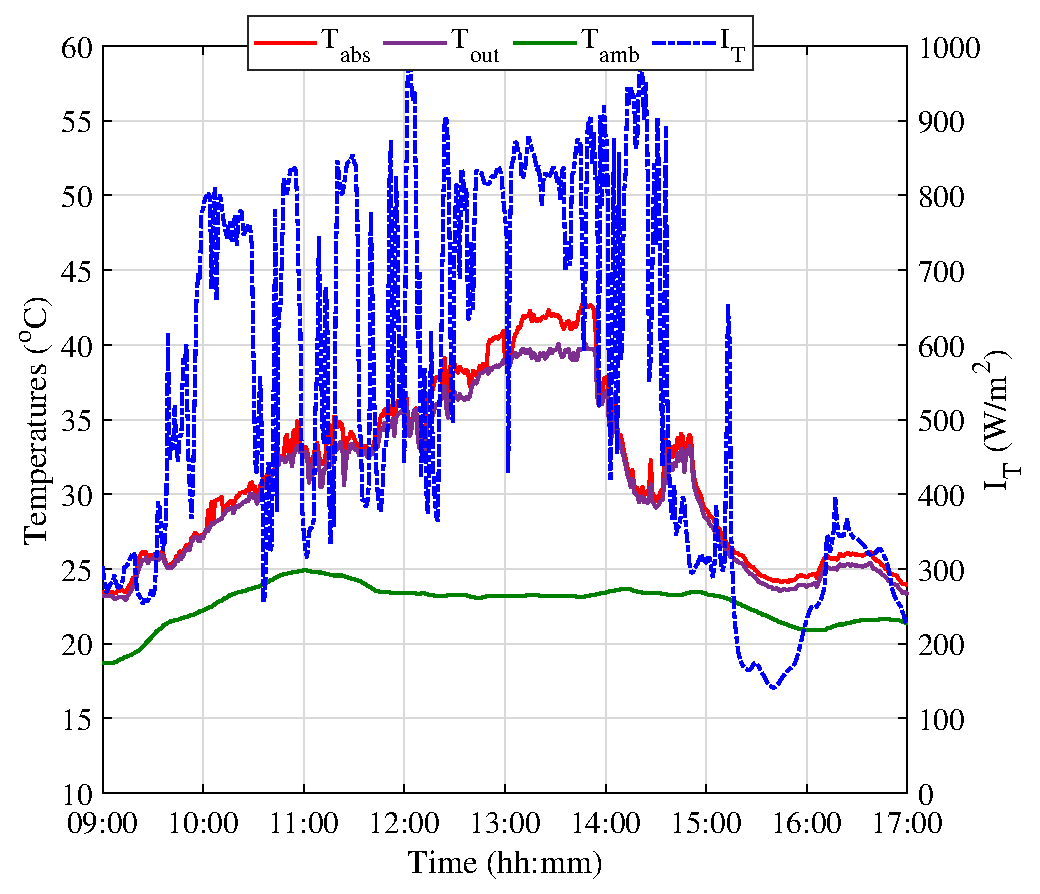
\includegraphics[width=0.98\textwidth]{figs/009-1.eps} % first figure itself
		\subcaption{Temperature results and solar data.}
	\end{minipage}\hfill
	\begin{minipage}{0.49\textwidth}
		\centering
		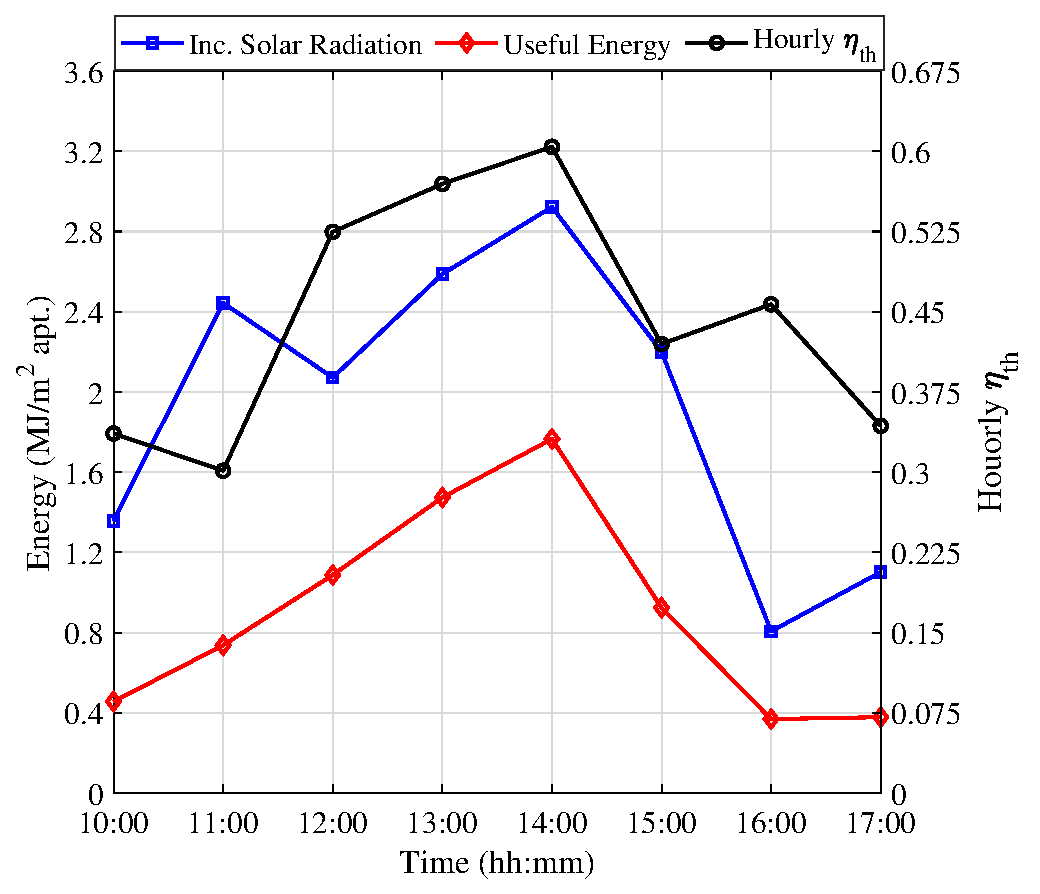
\includegraphics[width=0.98\textwidth]{figs/009-2.eps} % second figure itself
		\subcaption{Hourly performance and solar data.}
	\end{minipage}
	
	\caption{Experimental results from 31$^{\rm{st}}$ May at 0.089 kg/(s m$^2$).}
	\label{009}
\end{figure}

The results of a high airflow rate (0.114 kg/m$^2$.s) experiment are presented in Figure \ref{0115}. It was tested on June 28$^{\rm{th}}$ under clear sky conditions with the highest solar radiation values at the expected solar noon hour, where its peak was 850 W/m$^2$. During this hour, the average values of $\rm{T_{out}}$, $\rm{T_{amb}}$, and $\eta_{\rm{th}}$ were 38 $^{\rm{o}}$C, 27 $^{\rm{o}}$C, and 0.62, respectively. At around the peak of solar radiation, the maximum $\rm{T_{out}}$ was found to be 39 $^{\rm{o}}$C, resulting in the maximum airflow temperature rise of 12 $^{\rm{o}}$C and a corresponding $\eta_{\rm{th}}$ of 0.65. The total incident solar radiation during the test was estimated to be 21.07 MJ/m$^2$, of which the total useful energy collected $\rm{Q_{u}}$ was 9.8 MJ/m$^2$, resulting in a daily thermal efficiency of 0.47.

\begin{figure}[!ht]
	\centering
	\begin{minipage}{0.49\textwidth}
		\centering
		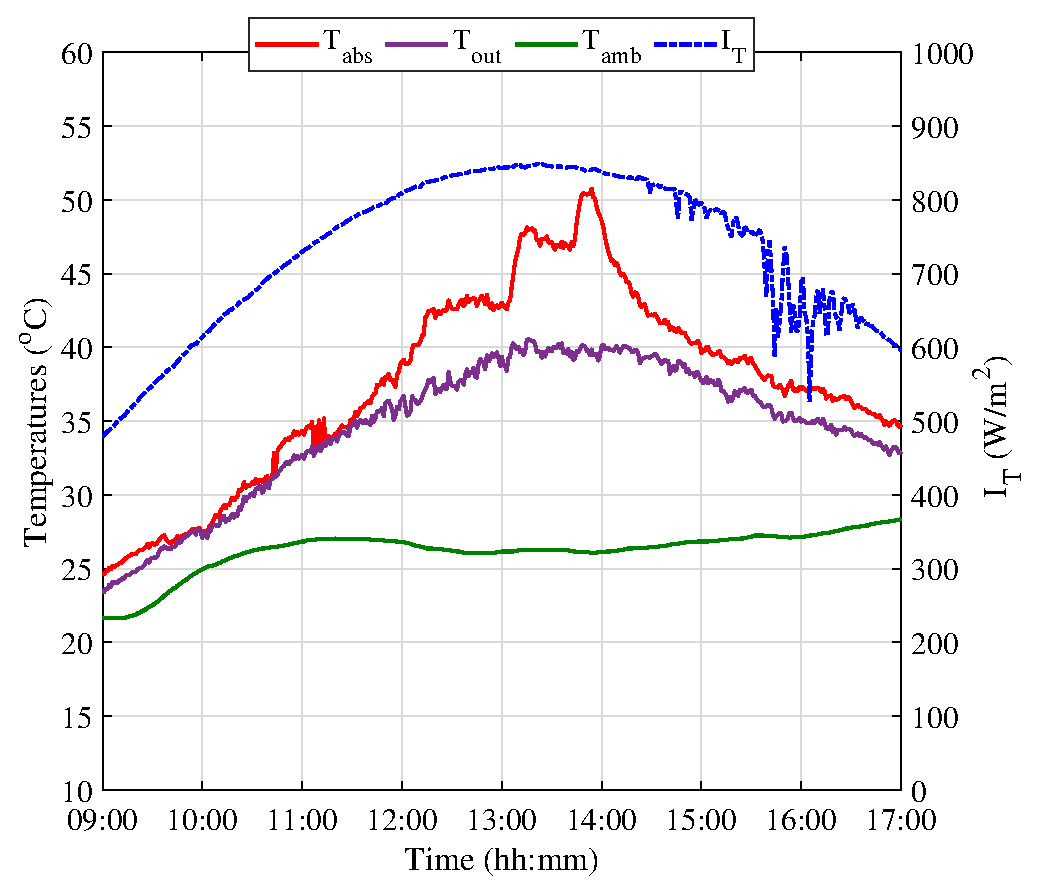
\includegraphics[width=0.98\textwidth]{figs/0115-1.eps} % first figure itself
		\subcaption{Temperature results and solar data.}
	\end{minipage}\hfill
	\begin{minipage}{0.49\textwidth}
		\centering
		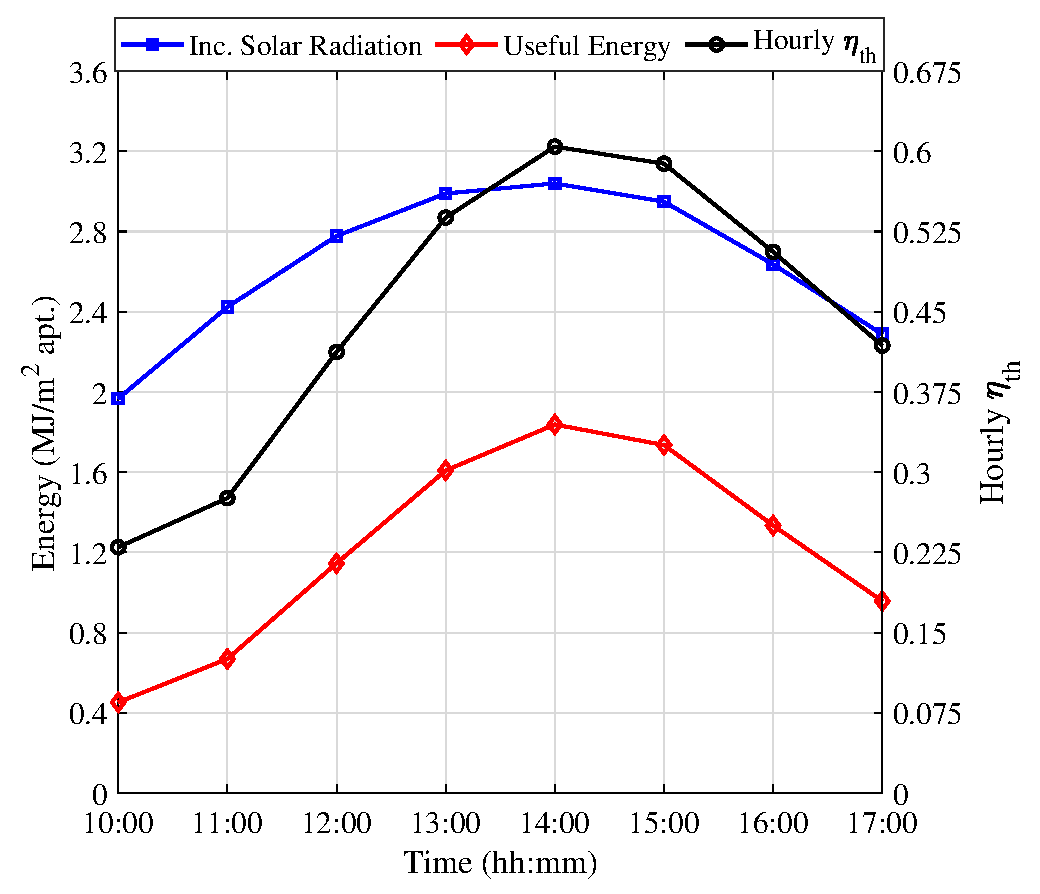
\includegraphics[width=0.98\textwidth]{figs/0115-2.eps} % second figure itself
		\subcaption{Hourly performance and solar data.}
	\end{minipage}
	
	\caption{Experimental results from 28$^{\rm{th}}$ June at 0.114 kg/(s m$^2$).}
	\label{0115}
\end{figure}

\newpage
\subsection{Experimental characterisation at nearly steady state}

The thermal characterisation of solar air heating relates the thermal efficiency under a steady state to each temperature rise normalised by the corresponding solar radiation according to the Hottel-Whillier-Bliss equation, expressed by Eq. (\ref{hottel-whiller-eq2}).

\vspace{-0.75cm}
\begin{equation}
\mathrm{\eta_{\rm{th}} = {F_{\!_R}}\eta_o - {F_{\!_R}}{U_{\!_L}}\frac{(T_{out} - T_{amb})}{I_{\!_T}}}
\label{hottel-whiller-eq2}
\end{equation}

\noindent where $\rm{F_{\!_R}}$ is the heat removal factor. From this equation, $\eta_{\rm{th}}$ can be plotted against $\rm{(T_{out} - T_{amb})/I_{\!_T}}$, resulting in a linear curve, with $\rm{F_{\!_R}}\eta_{\rm{o}}$ and $\rm{- F_{\!_R}{U_{\!_L}}}$ as the linear coefficient and the slope, respectively (\cite{Goswami2015}). 
%From this, the maximum thermal efficiency is $\rm{F_{\!_R}}\eta_{\rm{o}}$ when all the radiation absorbed is transferred to the airflow, but at no temperature change.

The experimental data collected for this analysis were during 10 minutes of tests around the solar noon period of clear days (nearly steady state condition), including all five airflow rates. This is when the direct radiation range is at a maximum of 800 -- 900~W/m$^{\rm{2}}$. To minimise the effects of the system's heat capacity, the data were taken in nearly symmetrical pairs, one before and one after noon, thus resulting in five averaged pairs for each day of experimental tests (\cite{Duffie2013}). Thermal efficiency was calculated by Eq. (\ref{ThermalEf0}). With all the data collected, the thermal efficiency curve was plotted in Figure \ref{ef_curve}. 

\Figure[scale=0.50,placement=!ht,label={ef_curve},caption={Hottel-Whillier-Bliss collector characterisation.}]{figs/exp_curve.eps}

\newpage
From these results, the parameters of Eq. (\ref{hottel-whiller-eq2}) were calculated: $\rm{F_{\!_R}}\eta_{\rm{o}}$ and $\rm{F_{\!_R}{U_{\!_L}}}$ are 0.652 $\pm$ 0.008 and -3.383 $\pm$ 0.328 respectively, and the coefficient of correlation is 0.8. It is important to state that $\rm{U_{\!_L}}$ is assumed to be weakly dependent on the absorber temperature in this operational range, where $\rm{(T_{out} - T_{amb})/I_{\!_T}}$ is between 0.015 and 0.037~m$^{\rm{2}}$.$^{\rm{o}}$C/W, so that the heat loss coefficient is constant (\cite{Rabl1985}). Compared to other work, \citet{Shams2016} characterised experimentally a solar air heating system with a similar geometry. They calculated the instantaneous thermal efficiency when the solar radiation varied between 937.6 and 1,085.4 W/m$^{\rm{2}}$. This resulted in a linear coefficient ($\rm{F_{\!_R}}\eta_{\rm{o}}$) of 0.73 and slope ($\rm{F_{\!_R}{U_{\!_L}}}$) of -3.25 W/m$^{\rm{2}}$.$^{\rm{o}}$C. The experimental results presented were influenced by varying ambient temperatures, as tests were conducted on days with different ambient conditions. The data were not normalized to account for these variations, which may have led to fluctuations in the observed response variables. Future studies could apply normalization techniques to improve comparison of results across different climatic conditions.

Next, Figure \ref{ef-Tout-Gair} shows thermal efficiency and outlet air temperature as functions of the mass airflow rate. From the thermal efficiency graph, it is possible to view a smooth increase in $\eta_{\rm{th}}$ when $\rm{G_{air}}$ becomes higher. The opposite behaviour is observed in the airflow temperature rise $(\rm{T_{out}} - \rm{T_{in}})$, where this variable dramatically drops when $\rm{G_{air}}$ varies from 0.04 to 0.09 kg/m$^2$.s and then falls smoothly by 2 $^{\rm{o}}$C.

\begin{figure}[ht!]
	\begin{minipage}{0.49\columnwidth}
		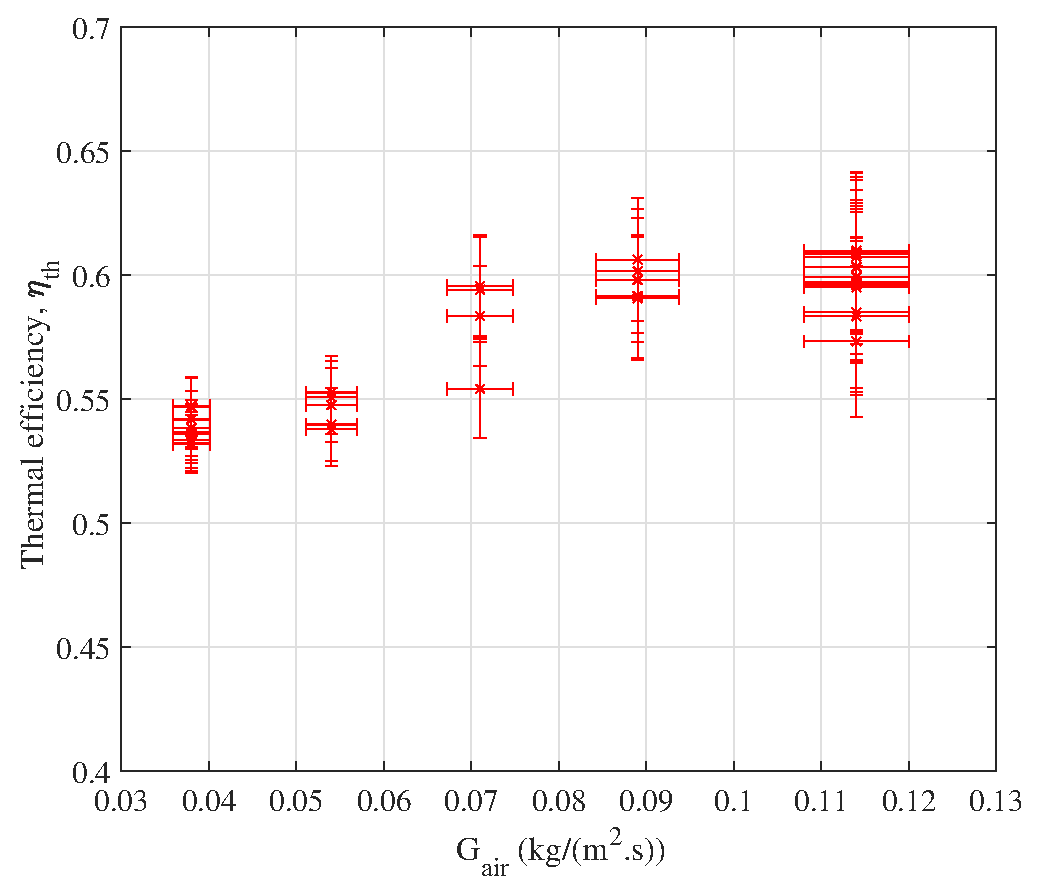
\includegraphics[width=0.98\columnwidth,height=6cm]{figs/ef-Gair2.eps}
		\subcaption{$\eta_{\rm{th}}$ vs. $\rm{G_{air}}$.}
	\end{minipage}
	\begin{minipage}{0.49\columnwidth}
		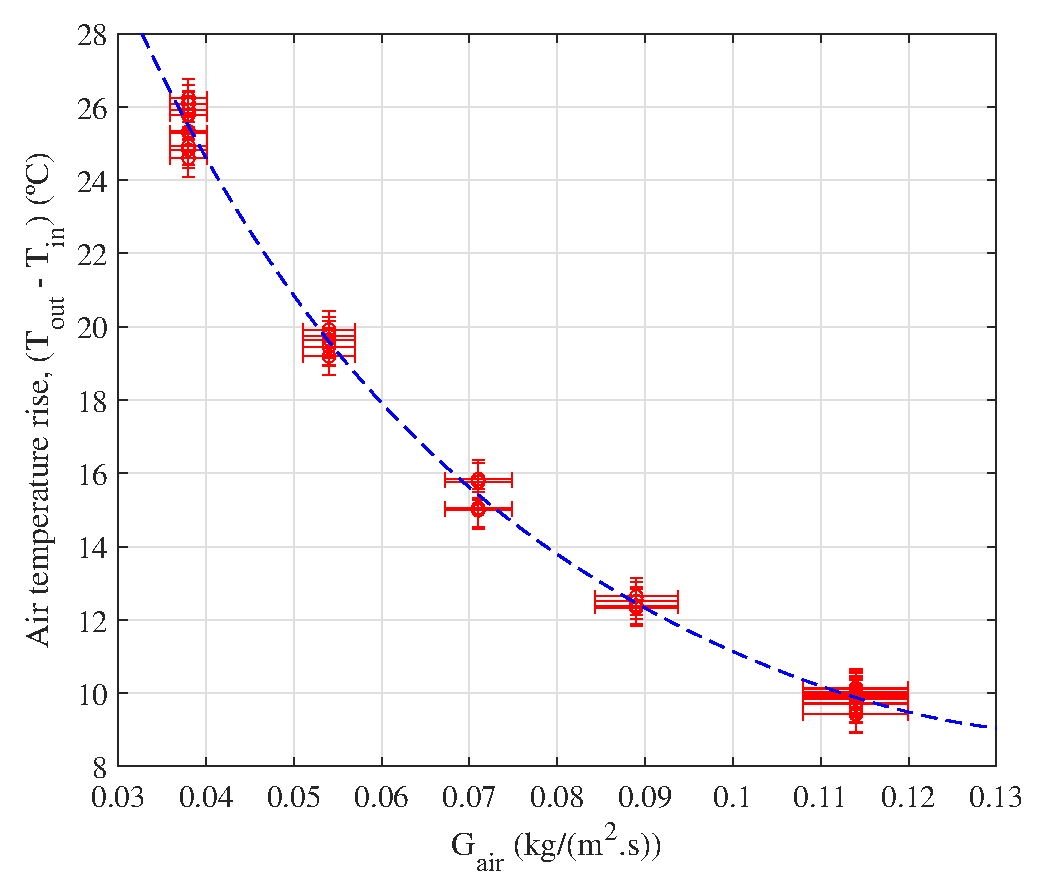
\includegraphics[width=0.98\columnwidth,height=6cm]{figs/dT-Gair2.eps}
		\subcaption{$\rm{(T_{out} - T_{in})}$ vs. $\rm{G_{air}}$.}
	\end{minipage}
    \caption{Graphs of thermal efficiency (a), and airflow temperature rise (b) at different airflow rates at nearly steady state condition.}
	\label{ef-Tout-Gair}
\end{figure}

%\subsection{Comparison of thermal performances}

%\citet{Koyuncu2006} tested 





\section{Chapter summary}

The fabrication of a solar air heating prototype for outdoor experimental tests has been detailed in this chapter. It outlined the selection of materials, the fabrication process and the data collection apparatus. Considering its material properties and the inherent perforation, carbon fibre weave with 85\% absorptivity was selected as the collector's absorber surface. 95\% reflectivity \textit{Mirosun} reflector sheet from the company Alanod was selected as the reflector material. A 4-mm thick tempered clear glass with 90\% transmittance was selected as the glazing cover.

The experiments were conducted in an open-loop configuration, where air was blown by a 12-W fan with a voltage adaptor to vary the airflow rate. Experimental results were obtained for airflow rates ranging from 0.038 to 0.115 kg/(m$^2$.s). Results show that the maximum outlet air temperatures at solar noon (13:00 to 14:00) varied from 40 $^{\rm{o}}$C at the highest airflow to 52 $^{\rm{o}}$C at the lowest and the thermal efficiency varied from 52\% to 62\%. 

Results were also evaluated at nearly steady-state conditions, where the maximum solar radiation range was at solar noon, 800 -- 900 W/m$^{\rm{2}}$. The thermal efficiency curve was plotted to characterise the system. The parameters of the Hottel-Whillier-Bliss equation were calculated: $\rm{F_{\!_R}}\eta_{\rm{o}}$ and $\rm{F_{\!_R}{U_{\!_L}}}$ are 0.65 and -3.39, respectively. The air temperature rise varied from 10~$^{\rm{o}}$C at the highest airflow rate to 26~$^{\rm{o}}$C at the lowest.






